%%%%%%%%%%%%%%%%%%%%%%%%%%
% BITTE IN UTF-8 OEFFNEN %
%%%%%%%%%%%%%%%%%%%%%%%%%%
\documentclass[xcolor=dvipsnames, compress, 10pt]{beamer}

\usepackage[ngerman] {babel}
\usepackage[ansinew] {inputenc}

\usepackage{tikz}
\usepackage{graphics}
\usepackage{BeamerColor}
\usepackage{expdlist} 
\usepackage{eurosym}

\usetheme{Warsaw}
\usefonttheme{professionalfonts}

\usecolortheme[named=ForestGreen]{structure}

\usepackage{ownTheme}
\setbeamertemplate{footline}[infolines theme]
\setbeamertemplate{headline}[miniframes theme]
\setbeamercovered{transparent=8}

%Code
\usepackage{listings}
%fuer fette typewriter Schrift
\renewcommand{\ttdefault}{pcr}

%Farben (benoetigt fuer listings)
\usepackage{color}
\usepackage[usenames,dvipsnames]{xcolor}

%vor jeder lstlisting-Umgebung aufrufen, 1. caption, 2. label
\newcommand{\javalstset}[2]{
\lstset{% general command to set parameter(s)
	basicstyle=\small\ttfamily, % print whole listing small
	keywordstyle=\color{DarkOrchid}\bfseries,
	% underlined bold black keywords
	identifierstyle=, % nothing happens
	commentstyle=\color{Gray}, % white comments
	stringstyle=\color{Blue}, % typewriter type for strings
	showstringspaces=false % no special string spaces 
	tabsize=3,
	language=Java,
	captionpos=b,
	caption={#1},
	label={#2},
	frame=trbl,
	breaklines=true,
	breakatwhitespace=true
	}
}

\AtBeginSubsection[]
{
\begin{frame}
\frametitle{}
\tableofcontents[currentsection]
\end{frame}
}

\begin{document}

\title[DLI Projekt: Kontakte]{DLI Projekt: Kontakte}
\subtitle[DLI]{Vorlesung Aktuelle Themen der Dienstleistungsinformatik}
%\date{\today} % gibt aktuelles Datum zurueck
\date{22. Januar 2013}
\author[M.\ Marzotko, T.\ Seeland, D. Wirkner]{Markus Marzotko, Thorben Seeland \& Dominic Wirkner\\ {\scriptsize Prof.\ Dr.\ Bernhard Steffen, Dipl.-Inf. Markus Doet}} 
\institute[TU Dortmund]{Technische Universit\"at Dortmund}

\nocite{*}

\frame{\titlepage}

\begin{frame}
%%%%%%%%%%%%%%	Gliederung		%%%%%%%%%%%%%%
\tableofcontents
\end{frame}			

\section{Einf\"uhrung}

\subsection*{Begriffskl\"arung}

\begin{frame}{Was ist Compliance?}
\pause
\begin{block}{Definition 1}
		\begin{quote}
			"`Die Binsenweisheit, dass Unternehmen Gesetze einhalten m\"ussen, hei{\ss}t nun
			Compliance."'
		\end{quote}
			Uwe H. Schneider, ZIP 2003, S. 645f
\end{block}
\pause
\begin{block}{Definition 2}
	\begin{quote}
		Bei "`Compliance"' geht es um die "`Erf\"ullung"', "`Entsprechung"' bzw.
		"`Konformit\"at"' mit staatlichen Gesetzen sowie mit Regeln und Spezifikationen,
		mit Grunds\"atzen (ethische und moralische) und Verfahren sowie mit Standards
		(z.B. ISO) und Konventionen, die klar definiert worden sind. Die Erf\"ullung der
		Compliance kann sowohl auf Zwang (z.B. durch Gesetze) als auch auf
		Freiwilligkeit (z.B. Einhaltung von Standards) beruhen.
	\end{quote}
		laut Compliance-Magazin.de
\end{block}
\end{frame}

\subsection*{Typische Anwendungsfelder}

\begin{frame}{Typische Anwendungsfelder}
\pause
\begin{itemize}[<+->]
	\item Medizin
		\begin{itemize}[<+->]
			\item ordnungsgem\"a{\ss}es Verschreiben von Medikamenten
			\item Befolgen der Ratschl\"age von \"Arzten
			\item Physiologie: Dehnbarkeit von K\"orperstrukturen
		\end{itemize}
	\item Cross-Compliance
		\begin{itemize}[<+->]
			\item landwirtschaftlicher Kontext
			\item betrifft Verpflichtungen f\"ur den Erhalt von EU-Direktbeihilfen:
				\begin{itemize}[<+->]
					\item landwirtschaftlicher und \"okologischer Zustand der Fl\"achen
					\item Futtermittel und Lebensmittelsicherheit
					\item Tiergesundheit und Tierschutz
				\end{itemize}
		\end{itemize}
	\item IT-Compliance
	\begin{itemize}[<+->]
		\item "`unsere"' Compliance
		\item Bedeutungsgewinn durch Digitalisierung von Gesch\"aftsprozessen
		\item Gesetze und Standards als Reaktion auf Computerpannen etc.
	\end{itemize}
\end{itemize}
\end{frame}

\section{Rechtliche Grundlagen}

\begin{frame}{Enron, Worldcom und Neuer Markt}
\begin{itemize}
	\pause
	\item \textbf{Enron} (USA, Energiekonzern)
	\pause
	\item \textbf{Worldcom} (USA, Telekommunikationskonzern)
	\pause
	\item \textbf{Neuer Markt}
\end{itemize}
\end{frame}

\subsection*{Sarbanes-Oxley Act}

%SAP 
\subsection{SAP Connector}

\begin{frame}
\begin{center}
\textbf{Aufgabe}

-Erhalte Kontaktobjekt mit Angaben zu Vorname, Nachname, Firma..
-Suche via Webservice und gefiltert nach den Daten 
-Gib aufbereitete Liste aller zutreffenden Kontakte zurück


\end{center}
\end{frame}

\begin{frame}
\begin{center}
\textbf{Programmablauf}

-Art des Filterobjekts überprüfen
-entsprechenden Webservice aufrufen
-IDs auslesen und anderen Webservice für alle IDs (einzeln) aufrufen
-Rückgabeobjekt auslesen und Daten zurückgeben
->Bei Mitarbeiter reicht erster Webserviceaufruf


\end{center}
\end{frame}

\begin{frame}
\begin{center}
\textbf{Problematik bei Lieferant und Kunde}

-Webservices geben hier nur Liste von IDs und Namen zurück
-Für Adressinformationen weiterer Aufruf mit anderem Webservice nötig
\textbf{PROBLEM:}Aufruf für jede ID einzeln

\end{center}
\end{frame}

\begin{frame}
\begin{center}

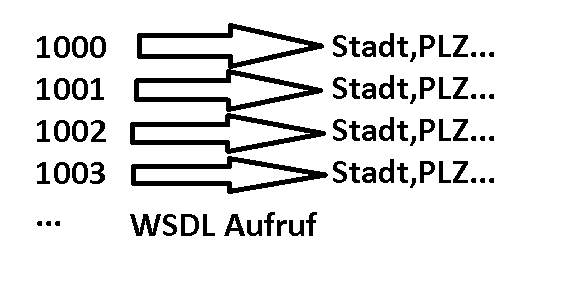
\includegraphics[width=\textheight]{Bilder/presi1.png} 

\end{center}
\end{frame}

\textbf{Lösung}
-GUI Darstellung so bauen, dass zunächst nur Name/Firma angezeigt werden
-Name/Firma werden bereits beim ersten Webservice Aufruf vorhanden
-


\begin{frame}
\begin{center}
\textbf{ProgrammablaufProblematik bei Lieferant und Kunde}


\end{center}
\end{frame}

-Was ist der ES-Workplace?

-Welche WSDLs wurden verwendet? Warum?

-Wie wurden die WSDLs ins Java Format übertragen? (WsImport..)

-Welche Probleme gab es bezüglich IDs und ``normalen Daten''?

-Was könnte diesbezüglich auf eigener Seite verbessert werden?



\begin{frame}
%%%%%%%%%%%%%%	Ende		%%%%%%%%%%%%%%
\begin{center}
Vielen Dank f\"ur die Aufmerksamkeit!
\end{center}
\end{frame}

\end{document}
